\chapter{Computer Vision} \label{chap:cv}

Importance of X-ray image analysis in pneumonia diagnoses clearly highlights that this is a computer vision problem. In essence computer vision is a scientific field aims to automate vision task usually performed by humans. Vision on earth begin approximately 543 million years ago when trilobites developed basic vision system~\cite{firstvision}. 
Development of vision helped increase the specie variation and development on earth significantly in respect to reproduction, finding food and many other reasons. Largely due to this very important nature of vision, research in how vision performed in species and how to automate the vision task gained a lot of attraction. Early research in this field inspired by the biological vision system. More specifically model of mammal neural system in respect to vision was the center point. In 1959 experiment on cat visual system by Hubel and Wiesel~\cite{hubel:single} highlighted the inner functioning of vision by discovering effect of dark edges causing activation in visual cortex. They also concluded that visual cortex passing this signals from detected edges to later centers of the brain where those edges are combined to represent more complex shapes. This idea of simple to more complex neural structure inspired Japanese computer scientist Kunihiko Fukushima to propose system he called \textit{Neocognitron}~\cite{fukushima:neocognitronbc}. In the article he laid out simple to complex neural architecture which was very similar to todays convolutional neural network (CNN).

\begin{figure}[H]%
    \centering
    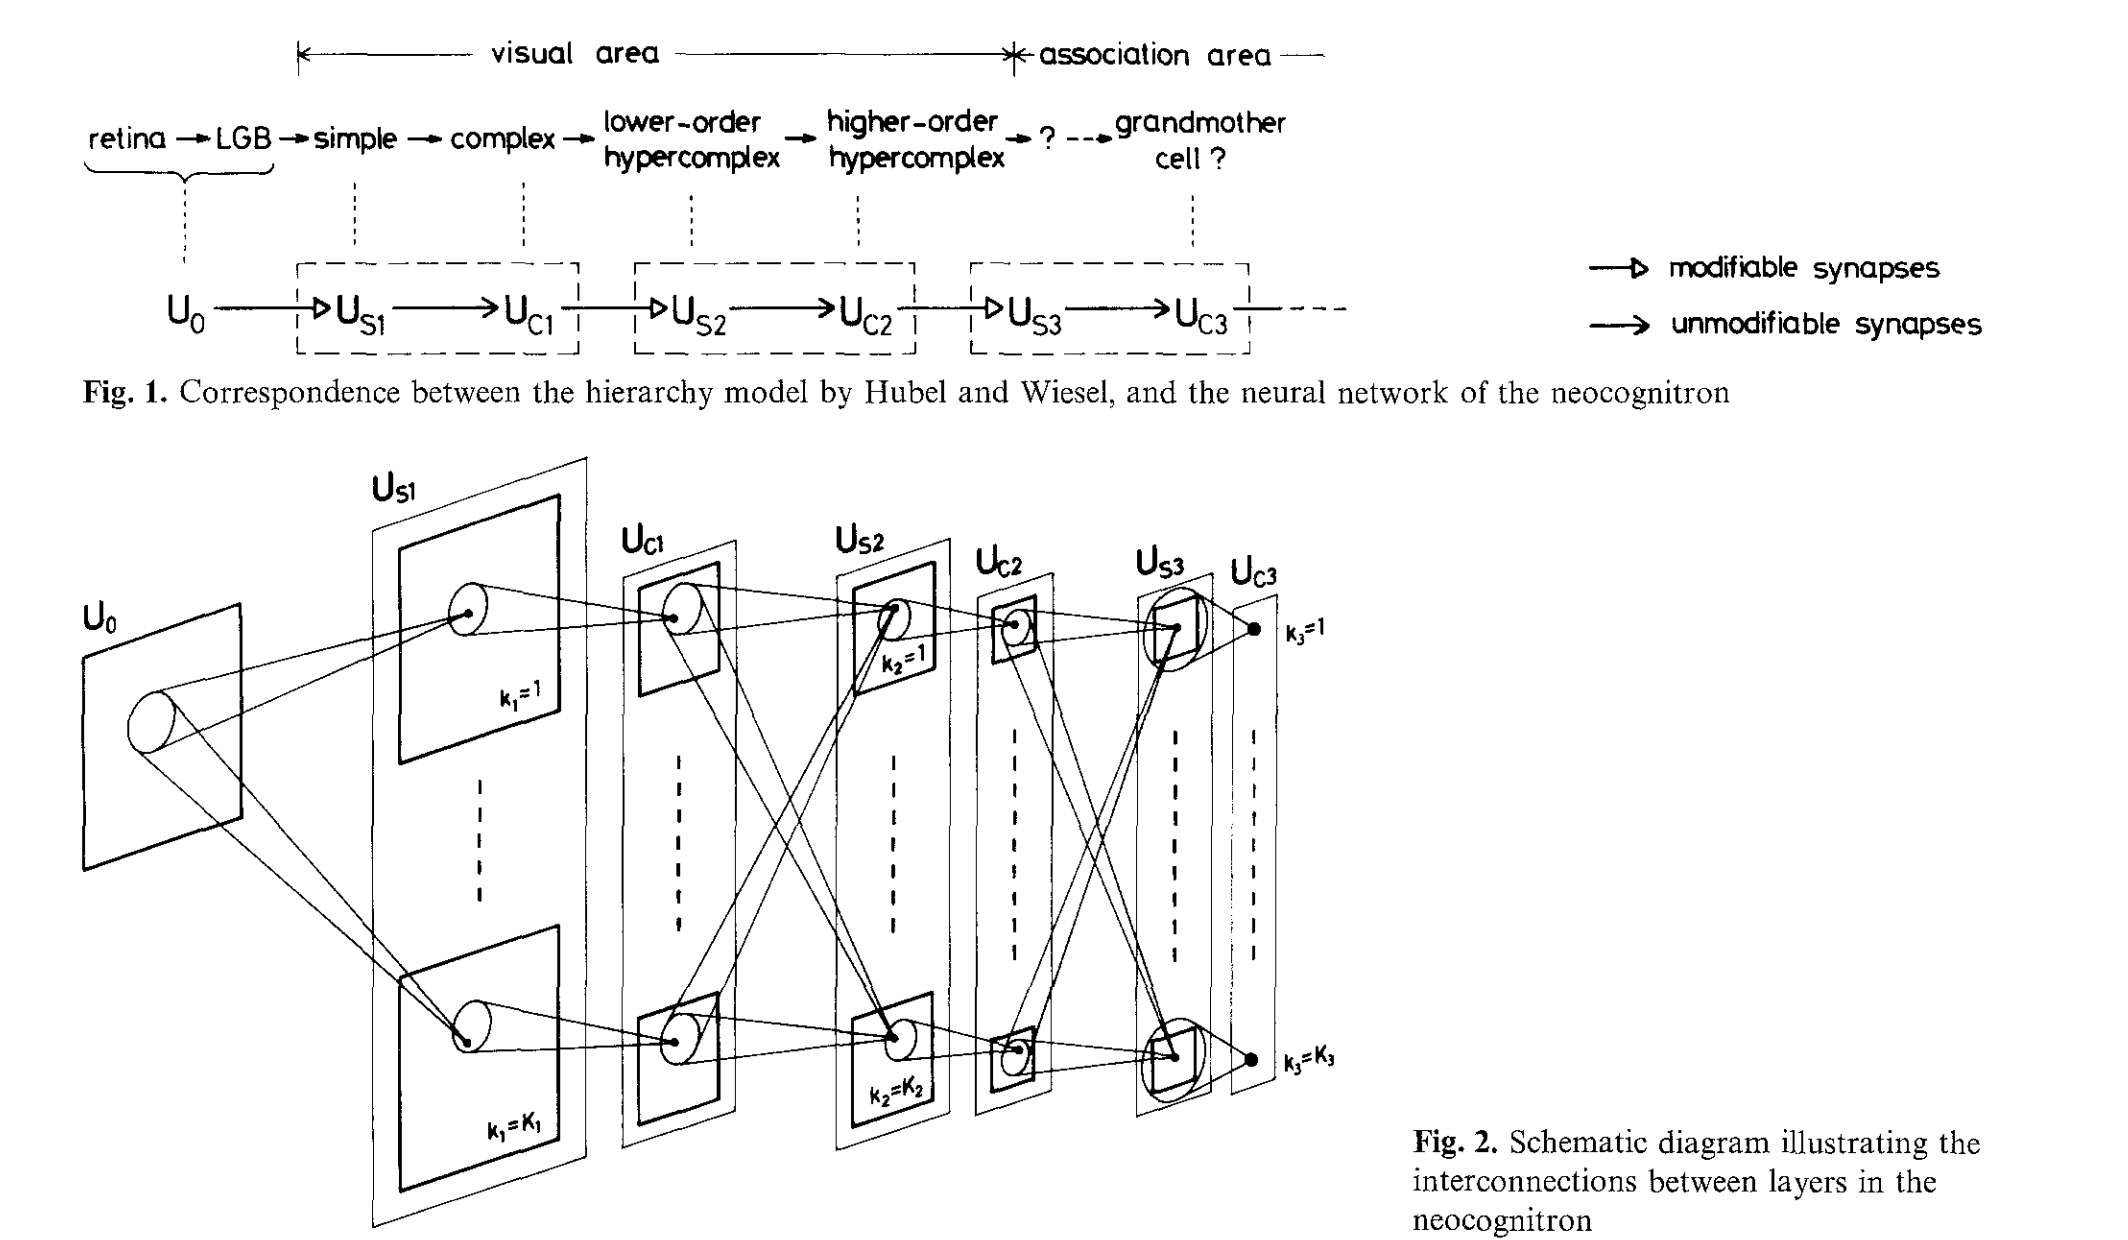
\includegraphics[width=\textwidth]{img/fukushima.png}%
    \caption{Network architecture from Neocognitron.}%
    \label{fig:neocognitron}%
\end{figure}

\section{Convolutional neural networks (CNN's)} \label{sec:cnns}
Although Neocognitron formed the general idea of the convolutional neural networks, it did not used the method called backpropagation that CNN's use today. Backpropagation is technique used in neural networks to propagate errors through the layers of neural network. First CNN that have the attributes same as current CNN's was build in Bell Labs in 1989 to recognize the hand written digits of the zip codes~\cite{cnnzipcodes}. Convolutional neural network name indicates that network uses mathematical operation called \textbf{convolution}. Explaining in a simple way using definition from the Deep Learning book~\cite{deeplearningbook}:

\begin{quote}
    "Convolutional networks are simply neural networks that use convolution in place of general matrix multiplication in at least one of their layers."
\end{quote}

Convolutional neural networks are generally a good option for image or time series data problems because of the sliding window approach capturing the underlying signal.

\section{Prominent computer vision architectures} \label{sec:prominentarch}
In this project I will be taking advantage of the well known network architectures for computer vision for general benchmarking purposes. These architecture generally known for their good performance in image classification competitions hence, any new design should perform better than these designs to be considered. 

\section{LeNet-5} \label{sec:lenet5}
LeNet-5~\cite{Lenet5} is 7 layered neural network build for classifying hand written digits in checks. Numbers in checks turned into  $32 \times 32$ pixel images and feed into the network for image classification task. LeNet-5 is the first successful application for combination of CNN and backpropagation. Network representation illustration and full specification of the network outlined below.

\begin{figure}[H]%
    \centering
    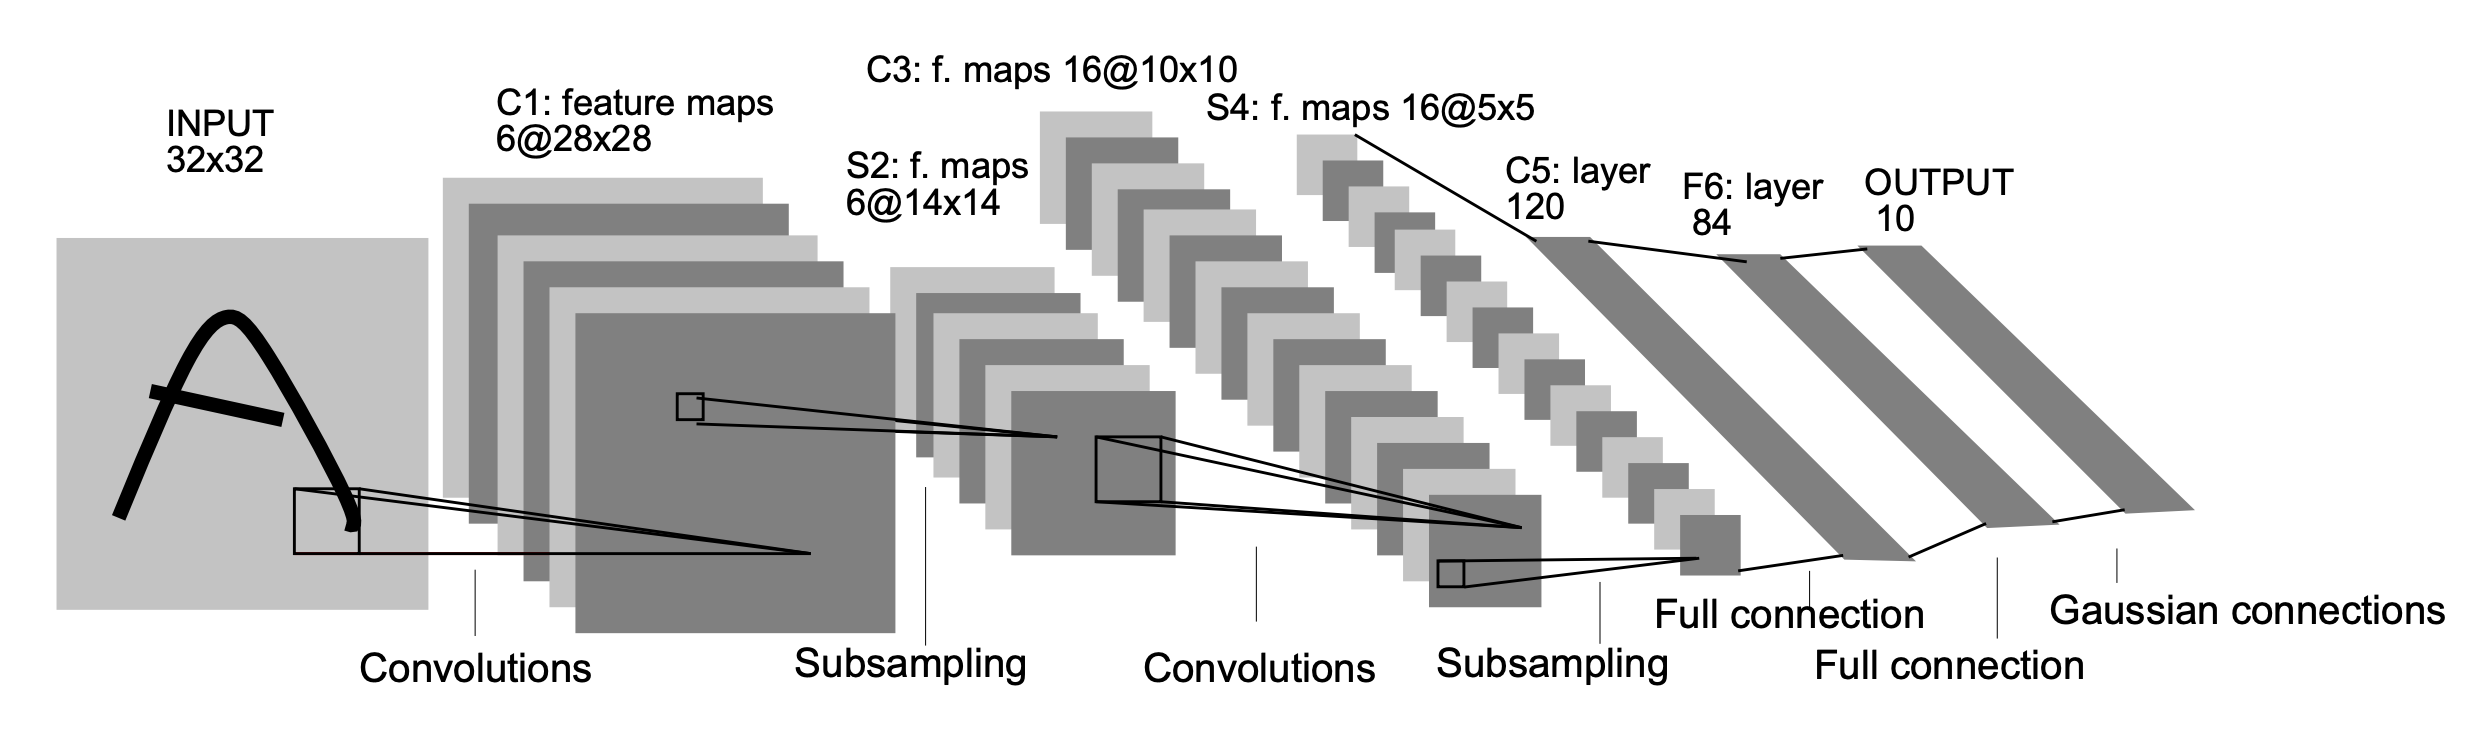
\includegraphics[width=\textwidth]{img/lenet-5.png}%
    \caption{Network architecture of LeNet-5.\\Credit: LeNet-5~\cite{Lenet5}}%
    \label{fig:lenet5}%
\end{figure}


\section{AlexNet} \label{sec:alexnet}
AlexNet~\cite{Alexnet} designed and named after Alex Krizhevsky, and published with collaboration of Ilya Sutskever and Geoffrey Hinton (advisor). It was designed for ImageNet challenge~\cite{imagenet} and utilized the idea of combining neural networks with graphics processing units (GPU) for high performance. This combination overcome the restriction of high computational demanding nature of neural networks and proved that current computational techniques are sufficient for training neural networks in even very large dataset such as the ImageNet. Another important implication is that AlexNet brought neural networks back to spotlight for research community after long break from LeNet-5's results. 

\begin{figure}[H]%
    \centering
    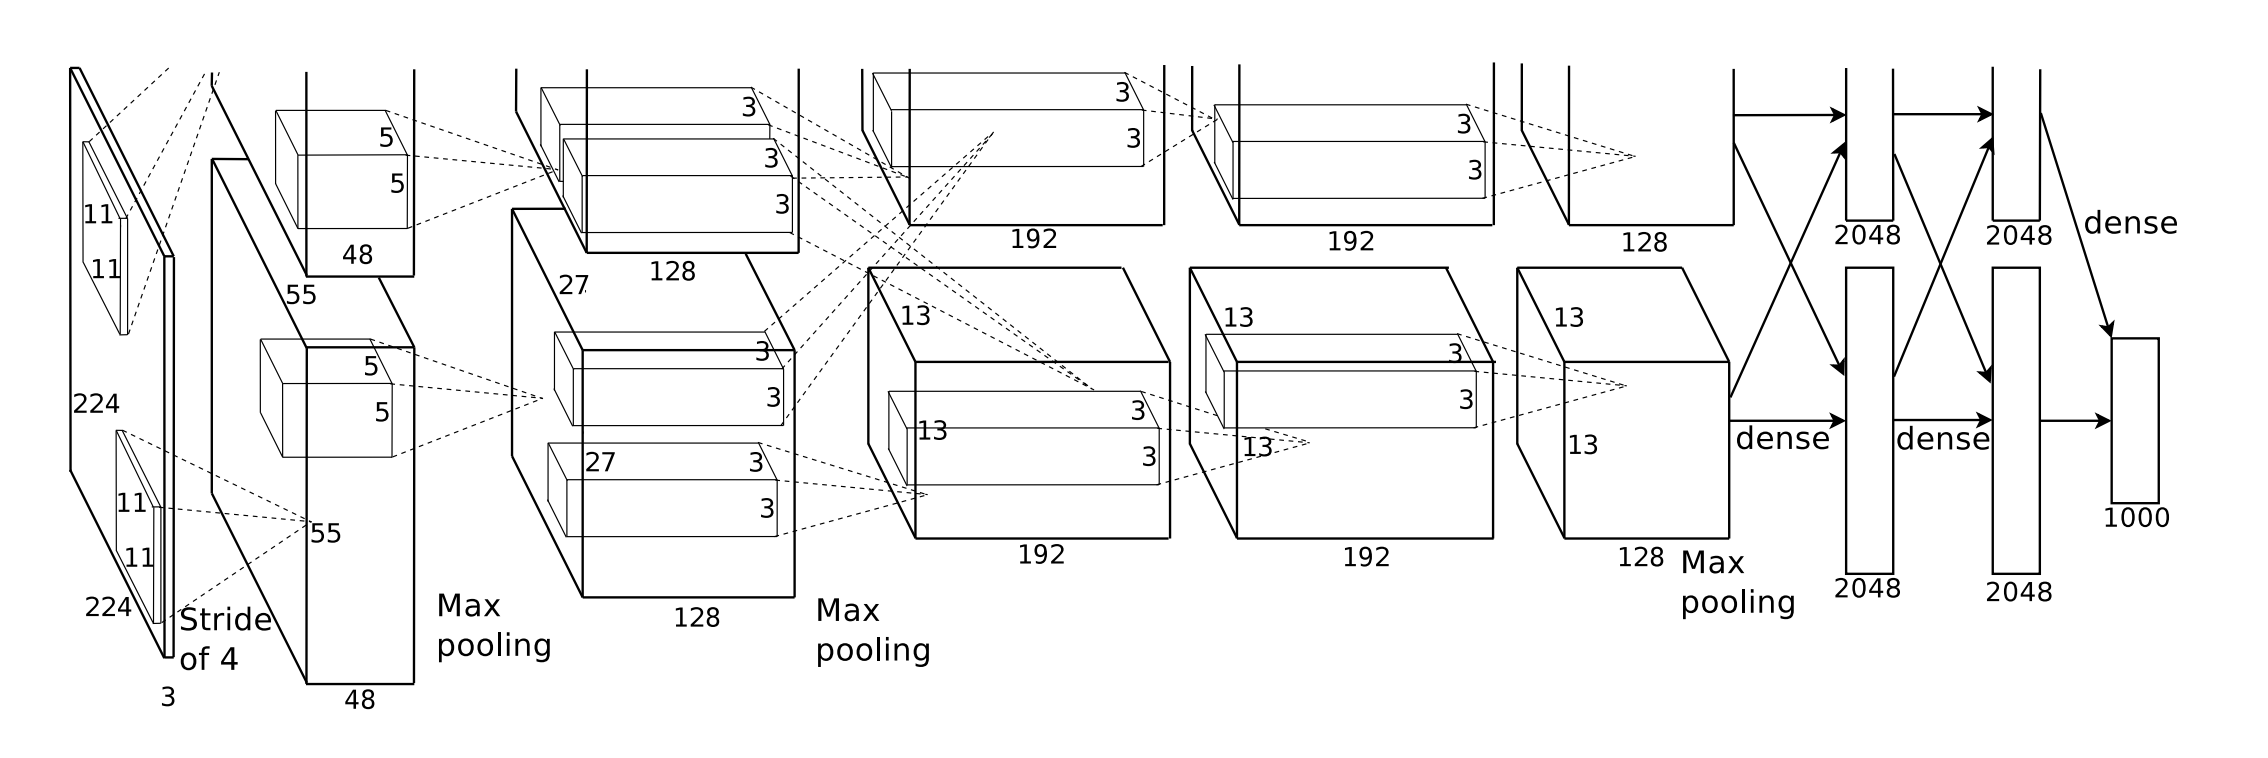
\includegraphics[width=\textwidth]{img/alexnet.png}%
    \caption{Network architecture of AlexNet.\\Credit: AlexNet~\cite{Alexnet}}%
    \label{fig:alexnet}%
\end{figure}

\section{VGGNet} \label{sec:vggnet}
VGGNet~\cite{vggnet} designed by Visual Geometry Group (VGG) from University of Oxford, this architecture also participated in ImageNet challenge~\cite{imagenet} for the year 2014. This research investigated the depth of the convolution neural networks effect on their accuracy. Doing so article walks through their general layout for experimenting different depth and characteristic of neural networks with comparison. Trial error approach they assumed, presents useful methodology for network prototyping this project will use. After obtaining high accuracy from this new deeper neural network inspired many similar high depth neural network architectures to be build. Success of these deep neural networks also get popular which lead the new popular term \emph{Deep Learning}.
\clearpage